% ---------------------------------------------------------------------------------------
%  Can We Trust the Answer?  --  RAG over Canadian pension-fund annual reports
%  Build:  cd report && latexmk -pdf report.tex      (or: pdflatex x2 + bibtex)
%  Figures/tables are generated by experiments/analyze.py from experiments/results/*.json
% ---------------------------------------------------------------------------------------
\documentclass[11pt,a4paper]{article}

\usepackage[utf8]{inputenc}
\usepackage[T1]{fontenc}
\usepackage{lmodern}
\usepackage[margin=2.4cm]{geometry}
\usepackage{microtype}
\usepackage{graphicx}
\usepackage{booktabs}
\usepackage{longtable}
\usepackage{tabularx}
\usepackage{array}
\usepackage{float}
\usepackage{caption}
\usepackage{subcaption}
\usepackage{enumitem}
\usepackage{amsmath}
\usepackage{xcolor}
\usepackage{pifont}
\usepackage{listings}
\usepackage{tcolorbox}
\usepackage{tikz}
\usetikzlibrary{positioning,arrows.meta,fit,backgrounds}
\usepackage{CJKutf8}
\usepackage{xurl}
\usepackage[colorlinks=true,linkcolor=blue!50!black,citecolor=blue!50!black,urlcolor=blue!50!black]{hyperref}
\usepackage[numbers,sort&compress]{natbib}

\definecolor{c1}{HTML}{2A78D6}
\definecolor{c2}{HTML}{EB6834}
\definecolor{c3}{HTML}{1BAF7A}
\definecolor{ink2}{HTML}{52514E}
\definecolor{boxbg}{HTML}{F6F7F9}

\newcommand{\cmark}{\textcolor{c3}{\ding{51}}}
\newcommand{\xmark}{\textcolor{c2}{\ding{55}}}
\newcommand{\hmark}{\textcolor{ink2}{\textonehalf}}
\newcommand{\R}[1]{\textbf{R#1}}

\captionsetup{font=small,labelfont=bf}
\setlist{itemsep=2pt,topsep=4pt}

% Q/A example boxes
\newtcolorbox{qa}[1]{colback=boxbg,colframe=ink2!40,boxrule=0.4pt,arc=2pt,left=6pt,right=6pt,top=4pt,bottom=4pt,
  fonttitle=\small\bfseries,coltitle=black,colbacktitle=ink2!12,title={#1}}
\newcommand{\Q}[1]{\noindent\textbf{Q:} \textit{#1}\par\smallskip}
\newcommand{\A}[1]{\noindent\textbf{A:} {\small\ttfamily #1}\par}

\lstset{basicstyle=\ttfamily\footnotesize,breaklines=true,columns=fullflexible,frame=single,
  rulecolor=\color{ink2!40},backgroundcolor=\color{boxbg},xleftmargin=4pt,xrightmargin=4pt}

\title{\textbf{Can We Trust the Answer?}\\[4pt]
\large Building and Validating a Multi-Source Retrieval-Augmented Generation Assistant\\
over Canadian Pension-Fund Annual Reports (HOOPP, AIMCo, OMERS)}
\author{Research project report \\ \small Repository: \url{https://github.com/lusinlusin/rag-investment-kb}}
\date{November 2026}

\begin{document}
\maketitle

\begin{abstract}
\noindent
Large pension funds and asset managers publish annual reports of 100--160 pages that mix narrative,
financial tables and infographics. Stakeholders --- trustees, investment committees, client-relations and
risk teams --- repeatedly ask the same kinds of questions of these documents: \emph{What did we return? Did we beat
the benchmark? How well funded are we? What did it cost?} A retrieval-augmented generation (RAG) assistant can
answer such questions in seconds, but in an investment setting a fluent, wrong number is worse than no answer.
This report documents an iterative study of a small, readable RAG system (local MiniLM embeddings, ChromaDB,
a DeepSeek LLM, a governed metric layer) over the 2025 annual reports of HOOPP, AIMCo and OMERS. We built a bank of
61 stakeholder-style questions with hand-verified gold answers plus 20 held-out questions, and ran seven rounds of
experiments in which each round responds to the failures of the previous one. Moving from one report to three
dropped accuracy from 91.3\% to 69.7\%; surprisingly, the cause was \emph{not} cross-fund contamination (about 98\% of
retrieved chunks came from the right organisation's report) but poor within-document recall and missing coverage for cross-fund questions.
Fund-aware routing alone did not help (71.3\%); hybrid BM25+dense retrieval did (91.8\%), and multi-query fusion
reached 95.9\% on the development set and 95.0\% on the held-out set (baseline 55.0\%). Validity stress tests show the
answers are grounded in the documents (97\% follow a deliberately edited number in the context), that naive
pipelines collapse on Chinese or abbreviated questions (12.5\% and 62.5\%) until a query-rewriting step is added,
and that the main residual risk is \emph{scope substitution} --- answering a neighbouring figure (a sub-portfolio, a
different fiscal date) when the requested one is absent. Every remaining error of the final system is an omission
or explicit refusal rather than an incorrect figure. We close with limitations and a concrete roadmap.
\end{abstract}

\tableofcontents
\newpage

% =====================================================================================
\section{Introduction}
\label{sec:intro}

\subsection{Motivation}
Canada's large public pension plans manage hundreds of billions of dollars on behalf of millions of members.
Each year they publish an annual report that combines a letter from the CEO, a management discussion and analysis
(MD\&A), performance tables by asset class, actuarial disclosures (funded status, discount rates, sensitivities),
cost disclosures and audited financial statements. The three reports used in this study are 108 (HOOPP), 98 (AIMCo)
and 156 (OMERS) pages long.

Inside an investment organisation, the people who need facts from these documents are rarely the people who
wrote them. A trustee preparing for a board meeting, an analyst benchmarking peers, a client-relations manager
answering a member's email or a risk officer checking a sensitivity all ask short, specific questions:
\emph{``What was the 10-year return versus benchmark?''}, \emph{``How exposed are we to the US dollar?''},
\emph{``Is HOOPP still fully funded?''}. Finding the answer means scrolling through the right report, the right
section and often the right table --- and then not confusing the Balanced Fund return with the Total Fund return,
or the smoothed funded ratio with the fair-value one.

Large language models (LLMs) can read and summarise text, but on their own they hallucinate, cannot cite, and
know nothing about documents published after their training cut-off. Retrieval-augmented generation
(RAG)~\citep{lewis2020rag,gao2023ragsurvey} addresses this by retrieving relevant passages from a document store
and asking the model to answer \emph{only} from them, with citations. RAG is therefore the natural architecture for
an ``ask the annual report'' assistant.

\subsection{Why validity is the central question}
In most consumer chat applications a slightly wrong answer is an inconvenience. In investment reporting it can be
a governance problem: a wrong return figure in a board pack, or one fund's funded ratio attributed to another, is
exactly the kind of error that erodes trust in an analytics function. The cost of errors is asymmetric: a refusal
(\emph{``I don't have that in the provided data''}) costs the user a minute of manual lookup, while a confident wrong
number may never be caught. We therefore evaluate the system less like a chatbot and more like a measurement
instrument: is it \emph{accurate}, is it \emph{grounded} in the documents, does it \emph{fail safely}, and are our
own accuracy numbers trustworthy?

\subsection{What this project does (the big picture)}
The starting point is a deliberately small RAG prototype (Section~\ref{sec:design}) that answered questions about
a single report (HOOPP 2025). The goal of this project is to find out what happens when that prototype is used the
way a real team would use it --- several organisations' reports in one knowledge base, questions phrased the way
stakeholders actually talk --- and to improve it round by round while checking that the improvements are real.
We ask four research questions:
\begin{description}[leftmargin=1.2cm,labelwidth=1cm]
  \item[RQ1] How accurate is the baseline pipeline on a single report, and where does it fail?
  \item[RQ2] What breaks when the knowledge base grows to three organisations' reports?
  \item[RQ3] Which interventions (fund-aware routing, contextual chunk headers, hybrid lexical retrieval, query
             rewriting, prompt rules) fix those failures --- and which do not?
  \item[RQ4] Are the answers \emph{valid}: grounded in the documents rather than model memory, robust to how
             stakeholders phrase questions (abbreviations, typos, Chinese), and able to say ``I don't know''?
\end{description}

\paragraph{Contributions.}
(i) A 61-question development bank and a 20-question held-out bank of stakeholder-style questions over three real
2025 annual reports, with hand-verified, regex-encoded gold answers and an audit log of every rubric change;
(ii) an evaluation harness that separates \emph{retrieval} failures from \emph{generation} failures via a
context-sufficiency metric, and that runs three validity stress tests (paraphrase, context ablation,
counterfactual editing); (iii) seven rounds of experiments with per-source (HOOPP / AIMCo / OMERS) results; and
(iv) practical findings, including two silent infrastructure pitfalls (approximate-nearest-neighbour misses and
PDF text artefacts) that would have biased the evaluation if left unchecked.

% =====================================================================================
\section{Background and Related Work}
\label{sec:related}
This is a project report rather than a paper, so we only sketch the work the design draws on.

\paragraph{Retrieval-augmented generation.}
\citet{lewis2020rag} introduced RAG as a combination of a dense retriever and a generator; \citet{gao2023ragsurvey}
survey the many variants that followed. Dense retrieval with bi-encoders was popularised by
DPR~\citep{karpukhin2020dpr}; our embedding model, \texttt{all-MiniLM-L6-v2}, is a small Sentence-BERT-style
encoder~\citep{reimers2019sbert} distilled with MiniLM~\citep{wang2020minilm}. Vector stores such as ChromaDB search
with approximate nearest-neighbour (ANN) indexes, typically HNSW~\citep{malkov2018hnsw}, which trade exactness for
speed --- a trade-off that turned out to matter here (Section~\ref{sec:r3}).

\paragraph{Lexical and hybrid retrieval.}
BM25~\citep{robertson2009bm25} remains a strong baseline for queries that hinge on exact terms and numbers.
Reciprocal rank fusion (RRF)~\citep{cormack2009rrf} is a simple, parameter-light way to merge ranked lists from
different retrievers, and is the fusion method we use. Query rewriting before retrieval~\citep{ma2023queryrewrite}
and prepending document-level context to chunks before embedding (``contextual retrieval'')~\citep{anthropic2024contextual}
are two recent, practical improvements that we test.

\paragraph{Financial question answering.}
FinQA~\citep{chen2021finqa} and TAT-QA~\citep{zhu2021tatqa} showed that numerical reasoning over hybrid
text-and-table financial documents is hard for language models; FinanceBench~\citep{islam2023financebench} found
that retrieval-augmented LLMs still answer many questions about public-company filings incorrectly. Our setting is
similar but narrower: institutional-investor annual reports and the questions their stakeholders ask.

\paragraph{Evaluating RAG and hallucination.}
\citet{ji2023hallucination} survey hallucination in natural-language generation. RAGAS~\citep{es2023ragas}
proposes reference-free RAG metrics (faithfulness, answer and context relevance) computed by an LLM.
\citet{chen2024rgb} benchmark LLMs on four RAG abilities --- noise robustness, \emph{negative rejection},
information integration and \emph{counterfactual robustness} --- which map closely onto our ablation and
counterfactual tests. \citet{liu2024lost} show that long contexts are not used uniformly, one reason we keep the
context short. Unlike LLM-judged metrics, we use deterministic, auditable regex grading against hand-built gold
answers, because a single wrong digit is the error we care most about.

% =====================================================================================
\section{Data}
\label{sec:data}

\subsection{Source documents}
All three documents are the organisations' official 2025 annual reports, downloaded as PDFs from their websites
(Table~\ref{tab:corpus}). They were chosen because they are comparable (Canadian, public-sector, multi-asset) yet
structurally different, which is exactly what stresses a multi-source assistant.

\begin{table}[H]
\centering\small
\caption{Corpus. Text chunks are 800-character windows with 150-character overlap; table chunks are tables recovered
by \texttt{pdfplumber} (one chunk per table). ``Pages w/ tables'' counts pages that yielded at least one table chunk.}
\label{tab:corpus}
\setlength{\tabcolsep}{4pt}
\begin{tabular}{lp{4.6cm}rrrr}
\toprule
Organisation & What it is & Pages & Text ch. & Table ch. & Table pages\\
\midrule
HOOPP & Healthcare of Ontario Pension Plan; DB plan, \$131.9B net assets, 109\% funded & 108 & 405 & 40 & 36\\
AIMCo & Alberta Investment Management Corp.; an \emph{investment manager} for Alberta public clients, \$194.7B AUM & 98 & 256 & 30 & 30\\
OMERS & Ontario Municipal Employees Retirement System; jointly sponsored DB plan, \$145.2B net assets & 156 & 529 & 68 & 56\\
\midrule
Governed metric layer & 8 versioned metric definitions (\texttt{data/metrics.yaml}) & -- & \multicolumn{3}{l}{8 metric chunks (never split)}\\
\bottomrule
\end{tabular}
\end{table}

\noindent Sources:
HOOPP \url{https://hoopp.com/docs/default-source/investments-library/annual-reports/hoopp-2025-annual-report.pdf};
AIMCo via \url{https://2025.annualreports.aimco.ca/} (``AIMCo-2025-AnnualReport.pdf'');
OMERS via \url{https://www.omers.com/2025-annual-report/highlights} (``OMERS\_2025\_AR.pdf'').
The PDFs are not redistributed in the repository.

\subsection{Structural differences that matter}
\begin{itemize}
  \item \textbf{Different kinds of organisation.} HOOPP and OMERS are pension plans with liabilities, a funded ratio
        and a discount rate. AIMCo is an asset manager: it has no plan-level funded ratio, so ``What was AIMCo's
        funded ratio?'' has no valid answer --- yet AIMCo's report does mention the funded status of \emph{its own
        employees'} supplementary plan, a perfect trap.
  \item \textbf{Several valid answers to one question.} AIMCo reports a \emph{Balanced Fund} return (7.6\%) and a
        \emph{Total AIMCo Fund} return (7.5\%); its ``private equity'' return is 3.0\% for the asset class but 4.5\%
        for the \emph{Core Private Equity} sub-portfolio; its corporate fiscal year ends March 31 while investment
        performance is reported to December 31. OMERS reports a smoothed (99\%) and a fair-value (96\%) funded ratio,
        and three different ``total benefits'' figures (\$6.8B in the highlights, \$6,584M and \$6,917M in Note 11).
  \item \textbf{Layout.} Highlights pages are infographics; financial tables are borderless; numbers are split by
        PDF text extraction (\texttt{7. 2 \%}, \texttt{1 1.4}, \texttt{Equities 3 7.0 \%}); OMERS uses an unusual
        thousands separator that \texttt{pypdf} renders as \texttt{81\textbf{?}621}; the OMERS highlights page
        yields a ``table'' whose numbers (\texttt{3.70\% 7.1\% 7.3\%}) have lost their labels.
\end{itemize}

\subsection{Evaluation questions}
\label{sec:questions}
We wrote questions the way stakeholders ask them (Table~\ref{tab:qbank}). The development bank has 61 questions:
15 per HOOPP, 12 AIMCo, 13 OMERS single-fund questions; 3 governed-metric questions; 6 cross-fund and 2
\emph{ambiguous} questions (no organisation named, e.g. \emph{``What was the net return in 2025?''}); and 10 traps ---
out-of-scope questions that must be refused (quarterly returns that are never reported, a 2026 forecast, a Sharpe
ratio or tracking error that the reports never state, a fund that is not in the corpus) and false-premise questions
that must be corrected (\emph{``Why did HOOPP's funded ratio fall below 100\%?''} --- it did not). A held-out bank of 20
further questions (15 single-fund, 1 cross-fund, 1 ambiguous, 3 traps) was written \emph{after} all seven rounds had
been designed and was only ever run on the baseline and final pipelines.

\begin{table}[H]
\centering\small
\caption{Question types, the stakeholder who typically asks them, and examples.}
\label{tab:qbank}
\begin{tabularx}{\textwidth}{lrlX}
\toprule
Type & Dev / HO & Typical asker & Example\\
\midrule
KPI lookup & 28 / 9 & Trustee, client relations & What were HOOPP's net assets at December 31, 2025?\\
Table lookup & 6 / 5 & Analyst & How did each of HOOPP's private-markets asset classes perform in 2025?\\
Reasoning & 3 / 0 & Investment committee & Which asset class contributed most to HOOPP's income, and what was its return?\\
People & 3 / 1 & Client relations & Who is AIMCo's CEO, and who chairs its Board?\\
Governed metric & 3 / 0 & Risk / performance team & What is our official definition of tracking error?\\
Cross-fund & 6 / 1 & Peer benchmarking & Compare the 2025 net returns of HOOPP, AIMCo and OMERS.\\
Ambiguous & 2 / 1 & Anyone & What was the funded ratio at the end of 2025?\\
Trap & 10 / 3 & (stress test) & Since AIMCo beat its benchmark in 2025, how large was the outperformance?\\
\bottomrule
\end{tabularx}
\end{table}

\paragraph{Gold answers.}
Every gold answer was looked up by hand in the PDFs, recorded with its page numbers, and encoded as one or more
\emph{groups} of regular expressions (\nolinkurl{experiments/questions.yaml}). An answer is correct only if it matches
at least one alternative in \emph{every} group --- e.g.\ question H01 requires both \texttt{7.7\%} (return) and
\texttt{8.6\%} (benchmark). Refusal questions are correct if the answer refuses or states that the data is not
available, and optional \texttt{forbid} patterns catch contamination (e.g.\ quoting HOOPP's 7.7\% as CPP
Investments' return).

% =====================================================================================
\section{System Design and Methodology}
\label{sec:design}

\subsection{Baseline pipeline}
Figure~\ref{fig:arch} shows the pipeline. It is intentionally small: each step is one Python file.

\begin{figure}[H]
\centering
\resizebox{\textwidth}{!}{%
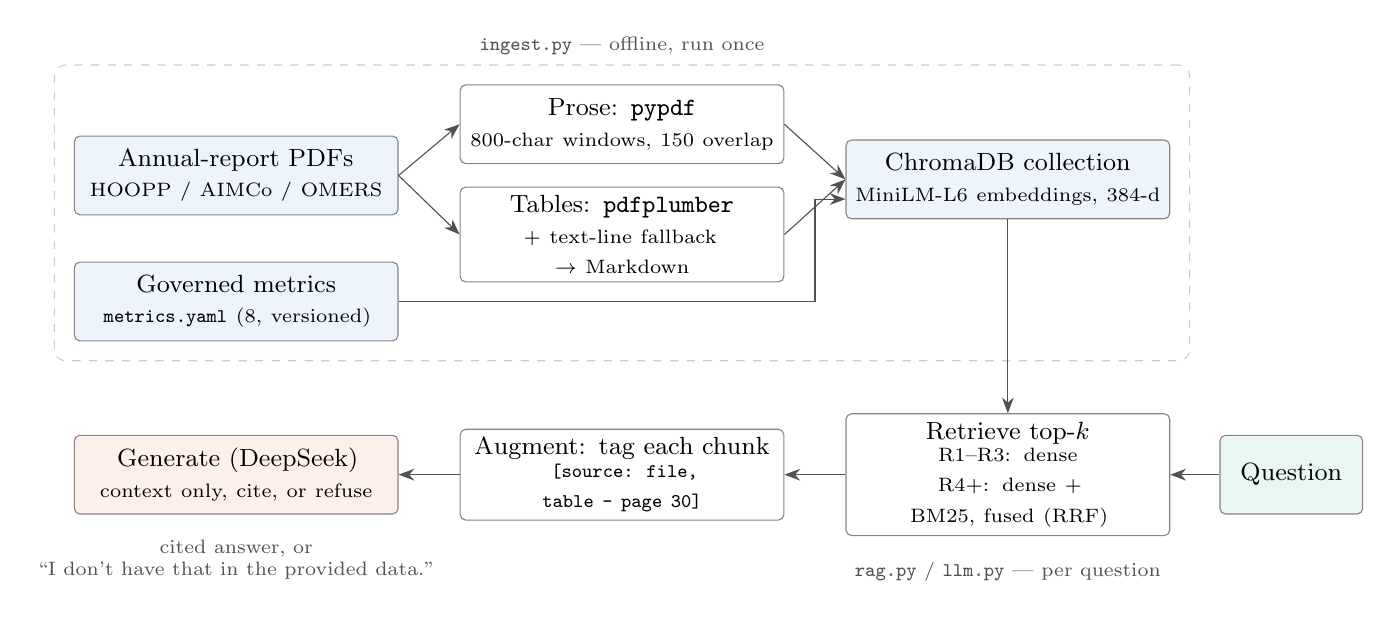
\begin{tikzpicture}[
  font=\small,
  box/.style={draw=ink2!70, rounded corners=2pt, fill=white, align=center, inner sep=3pt, minimum height=10mm, text width=39mm, execute at begin node={\hyphenpenalty=10000\exhyphenpenalty=10000}},
  data/.style={box, fill=c1!8},
  llm/.style={box, fill=c2!10},
  arr/.style={-{Stealth[length=2mm]}, ink2}]
% ---- offline ingestion (top row)
\node[data] (pdf)  at (0, 0.6)  {Annual-report PDFs\\\scriptsize HOOPP / AIMCo / OMERS};
\node[data] (yaml) at (0,-1.0)  {Governed metrics\\\scriptsize \texttt{metrics.yaml} (8, versioned)};
\node[box]  (prose) at (4.9, 1.25) {Prose: \texttt{pypdf}\\\scriptsize 800-char windows, 150 overlap};
\node[box]  (tab)   at (4.9, -0.15) {Tables: \texttt{pdfplumber}\\\scriptsize + text-line fallback $\to$ Markdown};
\node[data] (db)    at (9.8, 0.55) {ChromaDB collection\\\scriptsize MiniLM-L6 embeddings, 384-d};
\draw[arr] (pdf.east) -- (prose.west);
\draw[arr] (pdf.east) -- (tab.west);
\draw[arr] (prose.east) -- (db.west);
\draw[arr] (tab.east) -- (db.west);
\draw[arr] (yaml.east) -- (7.35,-1.0) |- ([yshift=-2.5mm]db.west);
\begin{scope}[on background layer]
\node[fit=(pdf)(yaml)(prose)(tab)(db), draw=ink2!30, dashed, rounded corners, inner sep=7pt,
      label={[font=\scriptsize,text=ink2]above:\texttt{ingest.py} --- offline, run once}] {};
\end{scope}
% ---- question time (bottom row, right to left)
\node[box, fill=c3!10, text width=16mm] (q) at (13.4,-3.2) {Question};
\node[box]  (ret) at (9.8,-3.2) {Retrieve top-$k$\\\scriptsize R1--R3: dense\\R4+: dense + BM25, fused (RRF)};
\node[box]  (aug) at (4.9,-3.2) {Augment: tag each chunk\\\scriptsize \texttt{[source: file,}\\\texttt{table - page 30]}};
\node[llm]  (gen) at (0,-3.2)   {Generate (DeepSeek)\\\scriptsize context only, cite, or refuse};
\draw[arr] (q) -- (ret);
\draw[arr] (db.south) -- (ret.north);
\draw[arr] (ret) -- (aug);
\draw[arr] (aug) -- (gen);
\node[below=2mm of gen, font=\scriptsize, text=ink2, align=center] {cited answer, or\\``I don't have that in the provided data.''};
\node[below=2mm of ret, font=\scriptsize, text=ink2] {\texttt{rag.py} / \texttt{llm.py} --- per question};
\end{tikzpicture}}
\caption{Pipeline. Ingestion builds one vector collection holding three chunk kinds (prose, tables, metric
definitions); question time is retrieve $\to$ augment $\to$ generate (\texttt{rag.py}).}
\label{fig:arch}
\end{figure}

\paragraph{Ingestion (\texttt{ingest.py}).}
Prose is extracted with \texttt{pypdf} and cut into 800-character windows with 150 characters of overlap. Because
\texttt{pypdf} flattens tables into ``number soup'', tables are extracted separately with \texttt{pdfplumber}
(text strategy), filtered to rows that look like data (a text label plus $\geq$2 numeric cells), rendered as
Markdown and prefixed with the surrounding prose so that they embed meaningfully; when the column grid fails, a
text-line fallback parses the page's clean lines. Each of the 8 governed metric definitions (tracking error,
Sharpe ratio, Brinson effects, \ldots) is one unsplit chunk carrying a version tag. Everything is embedded locally
with Chroma's default \texttt{all-MiniLM-L6-v2} (384 dimensions; no API key).

\paragraph{Retrieval, augmentation, generation (\texttt{rag.py}, \texttt{llm.py}).}
The question is embedded with the same model and the $k=6$ nearest chunks are returned. Each chunk is prefixed with
a source tag that distinguishes prose (\texttt{text}), tables (\texttt{table - page N}) and metric definitions
(\texttt{version: 1.0}). The LLM receives a strict system prompt (Appendix~\ref{app:prompts}): use only the
context, cite every fact by copying its tag verbatim, list multi-row answers as bullets, and reply exactly
\emph{``I don't have that in the provided data.''} when the answer is absent. The LLM is provider-agnostic; all
experiments use DeepSeek \texttt{deepseek-v4-flash} with the provider's default sampling settings.

\subsection{Experimental protocol}
The harness (\texttt{experiments/harness.py}) reuses the project's own functions (\texttt{ingest.load\_tables},
\texttt{ingest.chunk}, \texttt{rag.SYSTEM}, \texttt{llm.complete}), so every round evaluates the real pipeline and
changes only the component under study. Each round builds its own Chroma collection, retrieves for every question,
and asks the LLM \textbf{twice} (two repeats) to expose sampling variance. LLM responses are cached by
(system prompt, user prompt, repeat), so re-grading never re-queries the model; in total the study made
1{,}069 LLM calls. Round configurations are summarised in Table~\ref{tab:rounds}.

\begin{table}[H]
\centering\small
\caption{Round configurations. Each round changes one thing relative to its predecessor (R5 is a test round and
changes nothing). Questions: dev = 61-question development bank; HO = 20-question held-out bank.}
\label{tab:rounds}
\begin{tabularx}{\textwidth}{llX}
\toprule
Round & Corpus & Change (retriever / prompt) \\
\midrule
\R{1} & HOOPP & Baseline: dense top-6, prompt V1. 23 HOOPP / metric / trap questions.\\
\R{2} & 3 reports & Same pipeline, all three PDFs in one collection. 61 dev questions.\\
\R{3} & 3 reports & + contextual chunk headers, fund routing (filter / fan-out), prompt V2 (attribution rules), page-level citations.\\
\R{4} & 3 reports & + hybrid retrieval: dense + BM25 fused with RRF, $k=8$.\\
\R{5} & 3 reports & Validity stress tests on R4: paraphrase (casual, typo, Chinese), context ablation, counterfactual edit.\\
\R{6} & 3 reports & + LLM query rewriting before retrieval, prompt V3 (scope-strict, multilingual). Main set + stress tests.\\
\R{7} & 3 reports & Multi-query fusion: retrieve with original \emph{and} rewritten query. Main set, stress tests, held-out set.\\
\bottomrule
\end{tabularx}
\end{table}

\subsection{What we measure, and why}
\label{sec:metrics}
Our primary metric is \textbf{answer accuracy}: the fraction of answers (questions $\times$ repeats) that contain
every gold fact, or correctly refuse / correct the premise for traps. We deliberately did not use text-overlap
scores (BLEU/ROUGE) or an LLM judge as the headline: what matters to a stakeholder is whether the \emph{number} is
right, a regex check on the number is deterministic and auditable, and an LLM judge would introduce a second model
whose errors we would then need to validate. The secondary metrics each diagnose one failure mode:

\begin{itemize}
  \item \textbf{Context sufficiency} --- does the retrieved text, taken together, contain every gold fact? It is an
        upper bound on what generation can achieve and lets us split each error into a \emph{retrieval} error
        (insufficient context) or a \emph{generation} error (the answer was in the context but the model missed or
        refused it). It is lenient: co-occurrence of the right number is not proof that it is labelled correctly.
  \item \textbf{Fund purity} --- for single-fund questions, the share of retrieved document chunks that come from the
        right organisation's report; and \textbf{wrong-fund citation} --- the answer cites another organisation's
        report. Together they measure cross-source contamination, the risk we expected to dominate RQ2.
  \item \textbf{Invented source} --- a citation tag that does not correspond to any retrieved chunk.
  \item \textbf{False refusal} --- the model says ``I don't have that'' although the context was sufficient.
  \item \textbf{Repeat consistency} --- both repeats agree on correctness.
  \item \textbf{Validity stress tests} (R5--R7): \emph{paraphrase robustness} (8 questions $\times$ casual /
        typo / Chinese rewordings); \emph{context ablation} --- delete every retrieved chunk that contains the gold
        answer and check the model refuses (negative rejection~\citep{chen2024rgb}); and \emph{counterfactual
        editing} --- change the gold number inside the retrieved context (e.g.\ 7.7\% $\to$ 9.0\%) and check that the
        answer follows the context rather than the model's memory.
\end{itemize}
Statistical uncertainty is reported with 95\% bootstrap intervals over questions and exact sign tests on paired
per-question accuracy between rounds.

\subsection{Rubric audit}
Grading rules were fixed before each round, but reading the answers revealed cases where a ``wrong'' answer was
right. Each such change was logged (Appendix~\ref{app:audit}) and applied retroactively to \emph{all} rounds, so
every number in this report is computed with the same final rubric. Six changes were made to the development rubric
--- four accept a second, legitimate scope of the same figure (AIMCo Core Private Equity; AIMCo total costs including
third-party costs; OMERS benefits per Note 11; AIMCo excess return $-2.7\%$ as an equivalent of ``did not beat
the benchmark''), one removes a formula detail that the governed definition itself does not contain, and one stops
penalising a refusal that explicitly labels a related figure (\emph{``not reported; the full-year return was
7.7\%''}). One held-out item accepts the unit-equivalent \$4,096 million for \$4.1 billion.

% =====================================================================================
\section{Results and Analysis}
\label{sec:results}
Table~\ref{tab:main} and Figure~\ref{fig:rounds} summarise all rounds; the subsections below walk through them in
order. Figure~\ref{fig:fund} shows the same results broken down by source document.

\begin{table}[H]
\centering\small
\caption{Main results (development bank, two repeats per question, final rubric). Percentages are over answers
unless stated. ``--'' = not applicable (R1 has no cross-fund questions).}
\label{tab:main}
\begin{tabular}{lrrrrrr}
\toprule
Metric & R1 & R2 & R3 & R4 & R6 & R7 \\
\midrule
Questions $\times$ repeats & 23$\times$2 & 61$\times$2 & 61$\times$2 & 61$\times$2 & 61$\times$2 & 61$\times$2 \\
\textbf{Overall accuracy (\%)} & \textbf{91.3} & \textbf{69.7} & \textbf{71.3} & \textbf{91.8} & \textbf{91.0} & \textbf{95.9} \\
\quad Single-fund questions & 86.7 & 72.5 & 76.2 & 92.5 & 88.8 & 96.2 \\
\quad Cross-fund / ambiguous & -- & 12.5 & 12.5 & 75.0 & 87.5 & 87.5 \\
\quad Governed metrics & 100.0 & 100.0 & 100.0 & 100.0 & 100.0 & 100.0 \\
\quad Traps (refuse / false premise) & 100.0 & 95.0 & 90.0 & 100.0 & 100.0 & 100.0 \\
Context sufficiency (\%) & 88.9 & 68.6 & 72.5 & 86.3 & 88.2 & 94.1 \\
Accuracy $\mid$ sufficient context & 100.0 & 88.6 & 90.5 & 100.0 & 98.9 & 99.0 \\
False refusal $\mid$ sufficient context & 0.0 & 8.6 & 6.8 & 0.0 & 0.0 & 1.0 \\
Fund purity of retrieval (\%) & 100.0 & 97.9 & 100.0 & 100.0 & 100.0 & 100.0 \\
Wrong-fund citation (\%) & 0.0 & 0.0 & 0.0 & 0.0 & 0.0 & 0.0 \\
Invented source tag (\%) & 0.0 & 0.0 & 0.0 & 0.0 & 0.0 & 0.0 \\
Repeat consistency (\%) & 100.0 & 95.1 & 98.4 & 100.0 & 98.4 & 98.4 \\
Avg.\ chunks in context & 6.0 & 6.0 & 6.8 & 8.7 & 8.6 & 10.5 \\
\bottomrule
\end{tabular}

\end{table}

\begin{figure}[H]
\centering
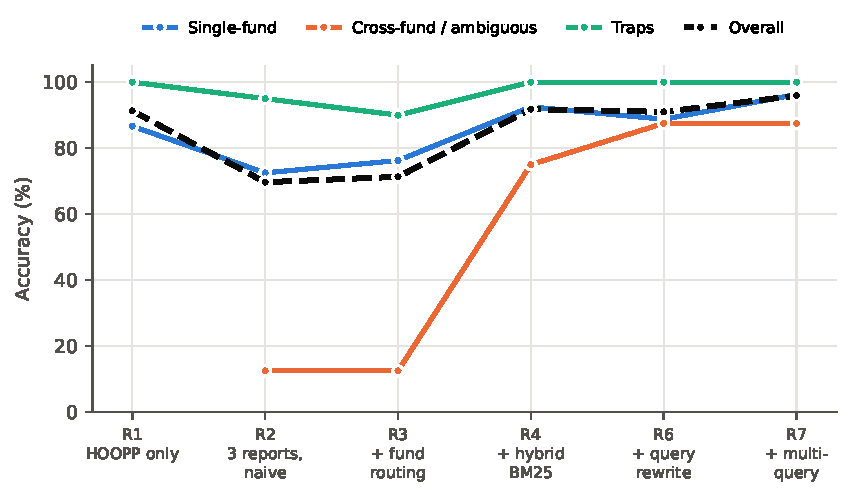
\includegraphics[width=0.86\textwidth]{figures/accuracy_by_round.pdf}
\caption{Accuracy by round and question group. Adding two reports (R2) hurts single-fund and especially
cross-fund questions; fund routing (R3) barely helps; hybrid retrieval (R4) recovers most of the loss; query
rewriting and multi-query fusion (R6--R7) close most of the remaining cross-fund gap.}
\label{fig:rounds}
\end{figure}

\begin{figure}[H]
\centering
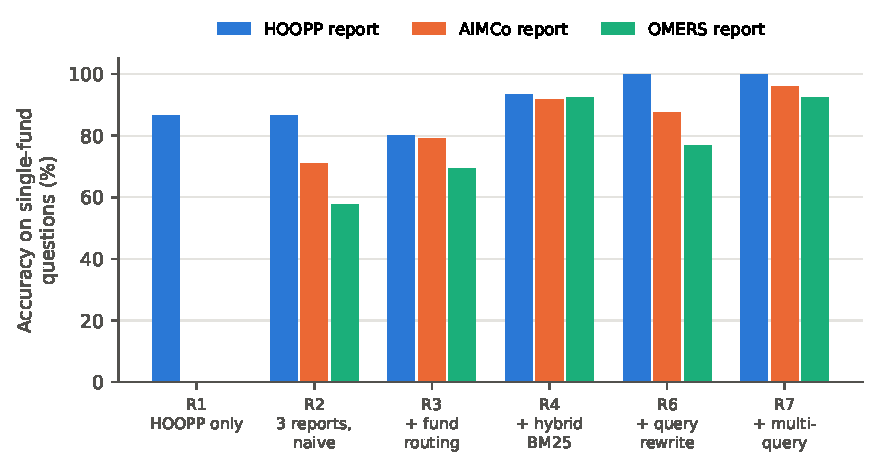
\includegraphics[width=0.86\textwidth]{figures/accuracy_by_fund.pdf}
\caption{Results by source document: accuracy on single-fund questions about each report (HOOPP $n=15$, AIMCo
$n=12$, OMERS $n=13$ questions, two repeats each). OMERS --- the longest, most table- and infographic-heavy report ---
is hardest throughout; R6 shows that query rewriting can \emph{hurt} one source (OMERS 76.9\%) while helping another.}
\label{fig:fund}
\end{figure}

% -------------------------------------------------------------------------------------
\subsection{Round 1 --- Baseline on a single report (HOOPP)}
\label{sec:r1}
\paragraph{Setup.} The original pipeline over the HOOPP report and the metric layer only (445 report chunks + 8
metric chunks); 23 questions: the 15 HOOPP questions, 3 governed-metric questions and 5 HOOPP-relevant traps.

\paragraph{Results.} Accuracy was \textbf{91.3\%} (42/46 answers). All traps were handled correctly (refusals for
the dog's name, a quarterly return, a 2026 forecast and a tracking error; a correction for the false
``funded below 100\%'' premise). Both repeats always agreed, every citation pointed to a retrieved chunk, and
whenever the context was sufficient the answer was correct (100\%). Typical answers look like this:

\begin{qa}{R1 --- table lookup and false-premise correction}
\Q{What was HOOPP's US dollar foreign currency exposure at the end of 2025 in Canadian dollars?}
\A{- United States Dollars: \$12,702 million (Canadian Dollar Equivalent) [source: hoopp-2025.pdf, table - page 84]}
\medskip
\Q{Why did HOOPP's funded ratio fall below 100\% in 2025?}
\A{The provided data does not show HOOPP's funded ratio falling below 100\% in 2025 --- it states the Plan was 109\% funded as of December 31, 2025. [...]}
\end{qa}

\paragraph{Failures.} The two failing questions are both \emph{retrieval} failures, and the model handled them
honestly. For H02 (\emph{``smoothed funded status at the end of 2025, and a year earlier?''}) the retriever found
the narrative saying the ratio ``declined modestly from 2024'' but not the page-21 table holding 111\%; the model
answered 109\% and said the 2024 value was not in the data. For H12 (\emph{``Have contribution rates changed
recently?''}) the sentence ``Contribution rates have not changed since 2004 and will remain [\ldots] until at least
the end of 2027'' was never retrieved, and the model refused. A third failure (M01) was a rubric error: we had
required the $\sqrt{12}$ annualisation detail that the governed definition does not contain (Appendix~\ref{app:audit}).

\paragraph{Is it valid, and what next?} The result looks good, but a single report is the easy case: every
retrieved chunk belongs to the right organisation, so the system cannot confuse sources. A real knowledge base
holds many organisations' documents. \emph{Next: add AIMCo and OMERS without changing anything else.}

% -------------------------------------------------------------------------------------
\subsection{Round 2 --- Naive multi-source knowledge base}
\label{sec:r2}
\paragraph{Setup.} The same pipeline over all three reports (1{,}328 report chunks + 8 metric chunks), evaluated on the
full 61-question development bank.

\paragraph{Results.} Accuracy fell to \textbf{69.7\%}. HOOPP questions were \emph{unaffected} (86.7\% in both R1 and
R2), but AIMCo (70.8\%) and OMERS (57.7\%) questions were much worse, and cross-fund / ambiguous questions collapsed
to 12.5\%.

\paragraph{The expected failure did not happen.} We expected the main risk to be \emph{contamination} --- an AIMCo
question answered with an OMERS number. It essentially never happened: fund purity was 97.9\%, and there were
\emph{zero} wrong-fund citations. Figure~\ref{fig:mix} shows why: when a question names the organisation, the small
embedding model picks up the name and retrieval stays on the right report.

\begin{figure}[H]
\centering
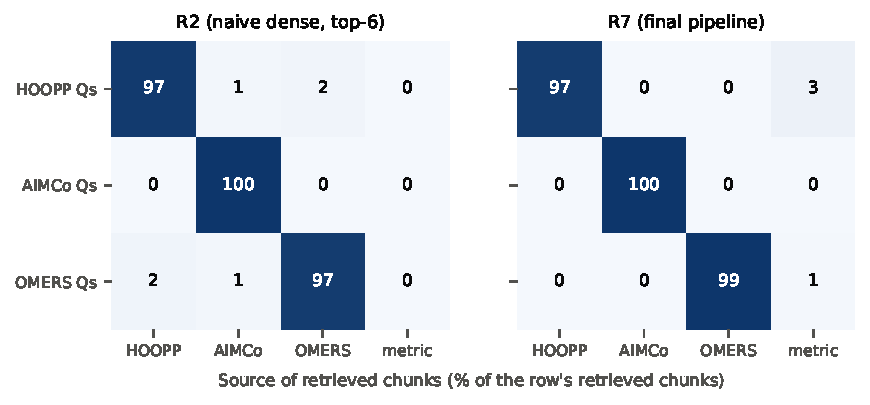
\includegraphics[width=0.82\textwidth]{figures/retrieval_source_mix.pdf}
\caption{Which report do retrieved chunks come from? Rows: questions about one organisation; columns: source of the
retrieved chunks. Even the naive R2 pipeline stays on the right report; cross-source contamination is not the
problem.}
\label{fig:mix}
\end{figure}

\paragraph{What did go wrong.} Context sufficiency dropped from 88.9\% to 68.6\%, and the failures fall into four
groups:
\begin{enumerate}
  \item \textbf{Within-document recall.} For AIMCo and OMERS the right report was searched but the right passage
        was not found: the management expense ratio (OMERS, ``58 basis points''), ``\$128.3 billion since
        inception'' (AIMCo), the 2025 benefits paid (OMERS). The model refused, correctly but unhelpfully.
  \item \textbf{Coverage for cross-fund questions.} Six chunks cannot cover three organisations. For
        \emph{``Compare the 2025 net returns of HOOPP, AIMCo and OMERS''} the context held HOOPP and OMERS, so the
        model reported those two and refused AIMCo.
  \item \textbf{Ambiguous questions answered for one fund.} This is the most dangerous answer in the round:
\begin{qa}{R2 --- an ambiguous question silently answered for one organisation}
\Q{What was the net return in 2025?}
\A{The net return in 2025 was 6.0\% [source: omers-2025.pdf, text].}
\end{qa}
        The number is correct for OMERS, and the citation reveals it --- but a reader who skims would take 6.0\% as
        ``the'' answer, while HOOPP returned 7.7\% and AIMCo 7.6\%/7.5\%.
  \item \textbf{Scope ambiguity in the source.} Asked for AIMCo's private-equity return and benchmark, the model
        answered 4.5\% vs 17.4\% --- the \emph{Core} Private Equity sub-portfolio on page 27 --- while the
        asset-class table gives 3.0\% vs 17.7\%. Asked for AIMCo's total costs vs budget, it answered \$1,157M vs
        \$1,207M (total costs including third-party costs) rather than \$425M vs \$490M (``Total AIMCo costs'').
        Both are grounded, cited and defensible; our rubric initially marked them wrong. Such cases are
        \emph{not} hallucinations, but they show that ``the right answer'' depends on a definition the user
        rarely states.
\end{enumerate}
Among answers with sufficient context, accuracy was still 88.6\%, with an 8.6\% false-refusal rate: the generator
sometimes refused when the number was present but poorly labelled (e.g.\ OMERS' highlights infographic reads
\texttt{3.70\% 7.1\% 7.3\%} with no labels attached).

\paragraph{Next.} Make retrieval fund-aware: tell the embedder which organisation each chunk belongs to (contextual
headers), filter retrieval to the named organisation, fan out across organisations for comparison and ambiguous
questions, and instruct the model to answer per organisation.

% -------------------------------------------------------------------------------------
\subsection{Round 3 --- Fund-aware retrieval and attribution rules}
\label{sec:r3}
\paragraph{Setup.} Three changes. (a) \textbf{Contextual headers:} each chunk is embedded with a prefix such as
\begin{center}\small\texttt{[OMERS (Ontario Municipal Employees Retirement System) - 2025 Annual Report - page 24] \ldots}\end{center}
(b) \textbf{Fund routing:} organisation names in the question are detected by pattern; one named fund $\Rightarrow$
metadata filter to that fund plus the metric layer; several $\Rightarrow$ 4 chunks from each; none $\Rightarrow$
the unfiltered top-6 plus the top-2 from every fund. (c) \textbf{Prompt V2}, which adds attribution rules (a fact
belongs only to the organisation in its tag; answer per organisation when none is named; correct false premises;
a metric definition is not a metric value), and citations that carry organisation and page for prose chunks.

\paragraph{Results.} Accuracy moved only from 69.7\% to \textbf{71.3\%} (6 questions improved, 4 worsened, sign test
$p=0.75$), and cross-fund accuracy stayed at 12.5\%. Purity rose to 100\%, but purity was never the problem.

\paragraph{Why it did not help: a retrieval-only study.} To understand the result without spending LLM calls we
measured context sufficiency for several retrieval strategies on the 51 answerable development questions
(Table~\ref{tab:study}, Figure~\ref{fig:study}). Headers and routing leave sufficiency at 69\%: they decide
\emph{which report} is searched, and the naive pipeline already got that right. What is missing is finding the
right \emph{passage} within the right report.

\begin{table}[H]
\centering\small
\caption{Retrieval-only study: context sufficiency (\%) by strategy (no LLM involved). ``Context'' is the mean
number of characters handed to the LLM.}
\label{tab:study}
\resizebox{\textwidth}{!}{\begin{tabular}{lrrrrrrr}
\toprule
Retrieval strategy & All & HOOPP & AIMCo & OMERS & Cross & Ambig. & Context (chars) \\
\midrule
dense k=6 (R2) & 66.7 & 86.7 & 58.3 & 69.2 & 16.7 & 50.0 & 5,054 \\
dense k=10 & 74.5 & 93.3 & 58.3 & 76.9 & 33.3 & 100.0 & 8,416 \\
+ context headers & 68.6 & 80.0 & 83.3 & 69.2 & 0.0 & 50.0 & 5,615 \\
+ fund routing (R3) & 68.6 & 80.0 & 83.3 & 69.2 & 0.0 & 50.0 & 6,413 \\
hybrid BM25 k=8, no headers & 82.4 & 100.0 & 75.0 & 84.6 & 33.3 & 100.0 & 7,105 \\
+ hybrid BM25 k=6 & 82.4 & 86.7 & 83.3 & 84.6 & 50.0 & 100.0 & 6,198 \\
+ hybrid BM25 k=8 (R4) & 86.3 & 93.3 & 83.3 & 92.3 & 50.0 & 100.0 & 7,759 \\
+ hybrid BM25 k=12 & 90.2 & 93.3 & 91.7 & 92.3 & 66.7 & 100.0 & 11,531 \\
\bottomrule
\end{tabular}
}
\end{table}

\begin{figure}[H]
\centering
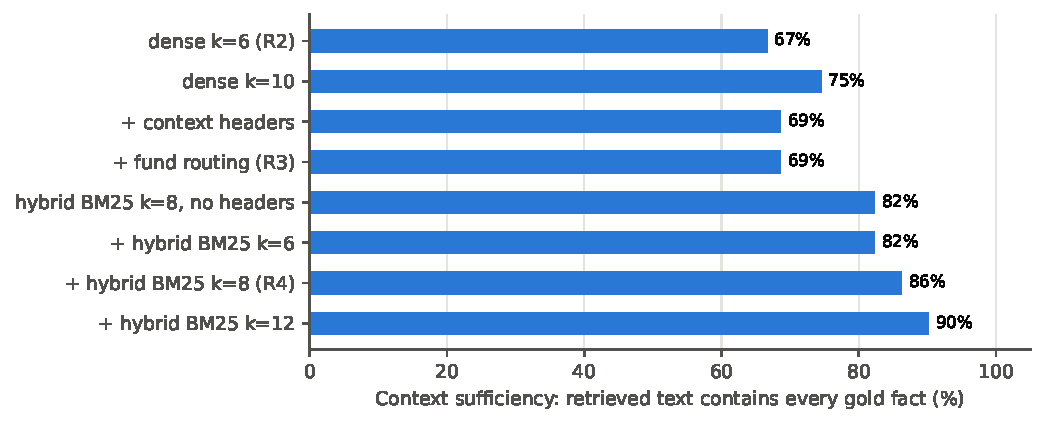
\includegraphics[width=0.8\textwidth]{figures/retrieval_study.pdf}
\caption{Context sufficiency by retrieval strategy. Lexical (BM25) evidence is the single largest lever; larger $k$
helps further but at the price of a longer context.}
\label{fig:study}
\end{figure}

\paragraph{A silent infrastructure pitfall.} While analysing R3, the governed-metric question \emph{``What is our
official definition of tracking error?''} started to fail: the tracking-error chunk was missing from the context.
Querying the collection with a filter showed that the chunk was the \emph{closest} vector to the question
(distance 1.064, better than any retrieved chunk) --- yet the unfiltered query did not return it. The cause is
Chroma's approximate HNSW index~\citep{malkov2018hnsw}: with default parameters (\texttt{ef\_search}=100,
\texttt{M}=16), once all report chunks shared a header prefix the eight metric vectors sat in an isolated region
the graph search did not reach. We measured ANN recall against exact brute-force search for every question:
it was 1.000 for the R1/R2 collections but 0.989 for the header collection, with misses on 2 of 61 questions
(one missing the exact top-1). Rebuilding all collections with \texttt{ef\_search}=\texttt{ef\_construction}=400,
\texttt{M}=32 restored recall to 1.000, and R3--R4 were re-run on the fixed index; all numbers in this report use
it. The lesson: an ANN index can silently drop the best evidence, and a 1{,}336-vector corpus would be better served by
exact search.

\paragraph{Next.} Add a lexical retrieval channel. The failing queries hinge on exact phrases and numbers
(``management expense ratio'', ``since inception'', ``pension benefits'') that a 22M-parameter sentence encoder
blurs, but BM25 matches directly.

% -------------------------------------------------------------------------------------
\subsection{Round 4 --- Hybrid lexical + dense retrieval}
\label{sec:r4}
\paragraph{Setup.} Within the same routing scheme, every search now runs BM25 (top-20) and dense retrieval
(top-20) over the same filtered chunks and fuses the two rankings with reciprocal rank fusion
($\text{score}=\sum 1/(60+\text{rank})$)~\citep{cormack2009rrf}; we keep the top $k=8$ (4 per fund for comparisons).
The retrieval study (Table~\ref{tab:study}) motivated the choice: hybrid at $k=8$ reaches 86\% sufficiency versus 82\% at
$k=6$ and 90\% at $k=12$ (which costs about 50\% more context).

\paragraph{Results.} Accuracy jumped to \textbf{91.8\%} (16 questions improved, 1 worsened vs R2, $p=0.0003$).
Single-fund accuracy rose to 92.5\% and was now nearly equal across sources (HOOPP 93.3\%, AIMCo 91.7\%, OMERS 92.3\%);
cross-fund accuracy rose from 12.5\% to 75\%; whenever context was sufficient the answer was correct (100\%, no false
refusals). Figure~\ref{fig:decomp} decomposes the errors: R2's losses were overwhelmingly retrieval errors, and R4
removes most of them.

\begin{figure}[H]
\centering
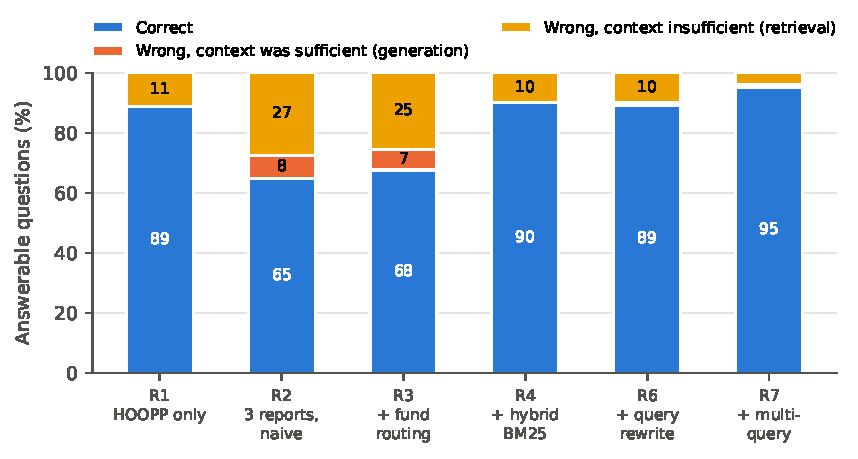
\includegraphics[width=0.86\textwidth]{figures/failure_decomposition.pdf}
\caption{Answerable questions split into correct, wrong despite sufficient context (generation error) and wrong
with insufficient context (retrieval error). From R4 on, generation is almost never the bottleneck.}
\label{fig:decomp}
\end{figure}

\paragraph{Too good to be true?} On paper, R4 matches the single-report baseline while handling three reports. But
the question bank is written in clean, fully spelled-out English that names each organisation --- exactly the
conditions under which retrieval is easiest --- and accuracy does not tell us whether the answers come from the
documents or from the model's memory, or what happens when the answer is missing. \emph{Next: stress-test validity
before improving anything else.}

% -------------------------------------------------------------------------------------
\subsection{Round 5 --- Validity stress tests}
\label{sec:r5}
\paragraph{Setup.} Three tests on the R4 pipeline (Table~\ref{tab:validity}, Figure~\ref{fig:validity}):
\begin{itemize}
  \item \textbf{Paraphrase robustness.} 8 development questions, each rewritten three ways: casual / abbreviated
        (\emph{``hoopp 2025 perf vs bmk?''}), typo-laden (\emph{``waht was HOOPPs net retrun in 2025 compared to
        benchmrak''}) and in Chinese (\begin{CJK*}{UTF8}{gbsn}``HOOPP 2025年的净回报率是多少？和基准相比如何？''\end{CJK*}).
  \item \textbf{Context ablation} (40 single-fund questions). Retrieve as usual, then delete every chunk that
        contains the gold answer (matched robustly to PDF spacing artefacts), and ask. The only correct behaviour is
        to refuse.
  \item \textbf{Counterfactual editing} (34 questions whose gold answer is a single number found in the context).
        Replace that number everywhere in the retrieved context with a perturbed value (+1.3 for decimals, e.g.\ HOOPP's
        7.7\% $\to$ 9.0\%) and ask. A grounded system must report the edited value.
\end{itemize}

\begin{table}[H]
\centering\small
\caption{Validity stress tests. R5 runs the tests on the R4 pipeline; R6 and R7 re-run them on their own pipelines
(case counts differ slightly because retrieval differs).}
\label{tab:validity}
\begin{tabular}{lrrr}
\toprule
Stress test & R5 (on R4) & R6 & R7 \\
\midrule
Paraphrase: casual / abbreviated (\%) & 62.5 & 100.0 & 100.0 \\
Paraphrase: typos (\%) & 87.5 & 100.0 & 75.0 \\
Paraphrase: Chinese (\%) & 12.5 & 100.0 & 87.5 \\
Paraphrase: all 24 (\%) & 54.2 & 100.0 & 87.5 \\
Ablation: refuses when answer removed (\%) & 75.0 & 85.0 & 80.0 \\
Counterfactual: follows edited context (\%) & 97.1 & 96.9 & 97.1 \\
Ablation cases (n) & 40 & 40 & 40 \\
Counterfactual cases (n) & 34 & 32 & 35 \\
\bottomrule
\end{tabular}

\end{table}

\begin{figure}[H]
\centering
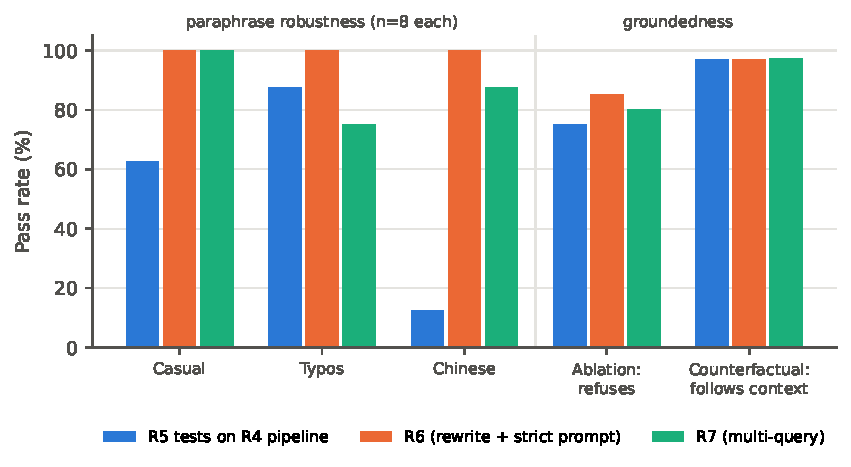
\includegraphics[width=0.86\textwidth]{figures/validity.pdf}
\caption{Validity stress tests across the last three pipelines.}
\label{fig:validity}
\end{figure}

\paragraph{Groundedness: good.} In 33 of 34 counterfactual cases (97.1\%) the answer reported the edited number,
and none reported the original --- strong evidence that answers come from the retrieved documents, not from the
model's memory of these 2025 reports. (The remaining case, AIMCo costs, answered with the alternative ``Total costs''
figure that we had not edited.) One example also exposes a weakness: after editing HOOPP's return to 9.0\% the model
reported \emph{``net return 9.0\%, benchmark 8.6\%, relative performance $-0.9\%$''} --- it copies figures without
checking that they are arithmetically consistent.

\paragraph{Negative rejection: the main residual risk.} With the answer removed, the model refused in 75\% of cases
(30/40). The other 25\% are the most important finding of this study: instead of refusing, the model
\emph{substituted a neighbouring figure} --- correctly cited and often correctly labelled, but answering a different
question:

\begin{qa}{R5 --- scope substitution when the requested figure is absent (ablation)}
\Q{How much were AIMCo's assets under management at the end of 2025?}
\A{At March 31, 2025, AIMCo's assets under management were \$180.8 billion [...] [source: aimco-2025.pdf (AIMCo), text - page 92]}
\medskip
\Q{What was OMERS's net return in 2025, and what was its benchmark?}
\A{For OMERS Public Equities: - Net Return: 12.3\% [...] - Benchmark: 7.6\% [source: omers-2025.pdf (OMERS), text - page 38]}
\end{qa}
The first answer gives a different date (AIMCo's fiscal year-end) and the second a sub-portfolio. A hurried reader
could easily take 12.3\% as OMERS' total-fund return. The three answers our first ablation filter flagged as
``memory leaks'' turned out to be filter artefacts (gold text split by PDF spacing or line breaks, e.g.\
\texttt{Annesley\textbackslash nWallace}, \texttt{7. 2 \%}); after making the filter whitespace-robust one remains, where
the context still contained the figures without a \% sign.

\paragraph{Paraphrase robustness: poor.} Only 13 of 24 paraphrased questions (54\%) were answered correctly:
typos were mostly harmless (87.5\%), abbreviations hurt (62.5\%: ``bmk'', ``PE'', ``fx''), and Chinese questions
failed almost completely (12.5\%) --- not because the LLM cannot read Chinese, but because the English-only MiniLM
embedder and BM25 cannot match a Chinese query to English text, so the context was irrelevant and the model correctly
refused.

\paragraph{Next.} (a) Rewrite each question into a clean, fully spelled-out English search query with the LLM before
retrieval; (b) tighten the prompt (V3): answer the exact metric, scope and date asked; if only a related figure exists,
refuse and name the related figure as different; name the variant (Balanced vs Total Fund, smoothed vs fair value)
for every figure; answer in the question's language.

% -------------------------------------------------------------------------------------
\subsection{Round 6 --- Query rewriting and a scope-strict prompt}
\label{sec:r6}
\paragraph{Setup.} Before retrieval, the LLM rewrites the question (prompt in Appendix~\ref{app:prompts}); the
rewritten query \emph{replaces} the original for retrieval, while the generator still sees the original question.
Prompt V3 replaces V2.

\paragraph{Results.} The stress tests improved sharply: paraphrase accuracy went from 54\% to \textbf{100\%}
(Chinese 12.5\% $\to$ 100\%), and refusal under ablation from 75\% to 85\%. But main-set accuracy slipped from 91.8\%
to 91.0\%, and per-source results diverged (HOOPP 100\%, AIMCo 87.5\%, OMERS 76.9\%; Figure~\ref{fig:fund}).
The diff is instructive: rewriting fixed some questions (H11, A05, X05 became sufficient) but broke others that
the original wording had retrieved well. For example, \emph{``Who is the President and CEO of OMERS?''} retrieved the
page with the CEO's full name under its original wording but not after rewriting, and the scope-strict model then
refused to guess:
\begin{qa}{R6 --- an honest failure caused by a rewritten query}
\Q{Who is the President and CEO of OMERS?}
\A{The context does not state the President and CEO's full name; it identifies the CEO only by the first name "Blake," [...] [source: omers-2025.pdf (OMERS), text - page 4]}
\end{qa}
Prompt V3 also changed how traps are answered: refusals now often name the related figure explicitly
(\emph{``I don't have that [\ldots] The context only reports an annual figure --- 2025 net return of 7.7\% [\ldots] --- not a
third-quarter return''}), which is the intended behaviour and prompted one rubric clarification.

\paragraph{Next.} Rewriting should \emph{add} evidence, not replace it. Retrieve with both queries and merge.

% -------------------------------------------------------------------------------------
\subsection{Round 7 --- Multi-query fusion (final pipeline)}
\label{sec:r7}
\paragraph{Setup.} Retrieve with the original question and with its rewrite (each through the R4 hybrid, routed
retriever), interleave the two ranked lists, de-duplicate, and keep at most $\max(|a|,|b|)+4$ chunks (10.5 on
average). Prompt V3.

\paragraph{Results on the development set.} \textbf{95.9\%} accuracy (bootstrap 95\% CI 91.0--100\%), the best of all
rounds: single-fund 96.2\%, cross-fund / ambiguous 87.5\%, traps 100\%, context sufficiency 94.1\%; per source HOOPP
100\%, AIMCo 95.8\%, OMERS 92.3\%. Relative to R2, 18 questions improved and none worsened ($p=7.6\times10^{-6}$).
Relative to R4 the main-set gain (3 questions improved, 0 worsened) is \emph{not} statistically significant
($p=0.25$); R7's advantage is robustness --- paraphrase accuracy 87.5\% versus 54\% for R4 (Chinese 87.5\%, casual
100\%, typos 75\%) --- while keeping groundedness (97.1\% follow the counterfactual edit) and a higher ablation-refusal
rate (80\% vs 75\%). The ambiguous question that R2 answered for one fund is now answered per organisation, with the
reporting variant named:

\begin{qa}{R7 --- the ambiguous question from R2, and a scope-ambiguous question}
\Q{What was the net return in 2025?}
\A{The net return for 2025 differs by organization:\\
- HOOPP: 7.7\% net return (2025) [source: hoopp-2025.pdf (HOOPP), text - page 29]\\
- OMERS: 6.0\% net return for 2025 (OMERS Primary Plan net return after all investment costs) [source: omers-2025.pdf (OMERS), text - page 5]\\
- AIMCo: 7.6\% Balanced Fund Net Investment Rate of Return (2025) [source: aimco-2025.pdf (AIMCo), text - page 3]\\
- AIMCo: 7.5\% Total AIMCo Net Investment Rate of Return [source: aimco-2025.pdf (AIMCo), text - page 3]}
\medskip
\Q{What was AIMCo's private equity return in 2025, and its benchmark?}
\A{AIMCo reports two variants:\\
- Core Private Equity: 4.5\% return in 2025; benchmark return 17.4\%; excess return (12.9)\% [source: ... page 27]\\
- Private Equity: 3.0\% return in 2025; no benchmark for this broader "Private Equity" figure is stated in the provided context [source: ... page 14]}
\end{qa}

\noindent And the same pipeline answering a Chinese question in Chinese:
\begin{qa}{R7 --- Chinese question (paraphrase test)}
\begin{CJK*}{UTF8}{gbsn}
\Q{HOOPP 2025年的净回报率是多少？和基准相比如何？}
\A{- 2025年净回报率（Net return）：7.7\% [source: hoopp-2025.pdf (HOOPP), text - page 29]\\
- 基准（Benchmark）：8.6\% [source: hoopp-2025.pdf (HOOPP), text - page 29]\\
- 相对表现（Relative performance）：-0.9\% [source: hoopp-2025.pdf (HOOPP), text - page 29]}
\end{CJK*}
\end{qa}

\paragraph{Remaining errors are safe errors.} The five failing development answers (A05 once, O07 twice, X06 twice)
and the two failing held-out answers (HO17) have one thing in common: each states that a figure is \emph{not in the
context} --- the infrastructure benchmark, the rest of OMERS' target mix (the chunk is cut mid-list after ``Public
Equities 19.0\%''), OMERS' benchmark in a three-way comparison, OMERS' net assets in an ambiguous question. None
reports an incorrect number.

\paragraph{Held-out check.} Because every design decision in R3--R7 was made by looking at the development
questions, the gains could be over-fitted to them. On the 20 held-out questions, written afterwards and never
used for tuning, the baseline (R2 pipeline) scored 55.0\% and the final pipeline \textbf{95.0\%} (8 questions improved,
0 worsened, $p=0.008$; Table~\ref{tab:heldout}). The improvement transfers.

\begin{table}[H]
\centering\small
\caption{Held-out evaluation: baseline vs final pipeline on 20 questions never used for design.}
\label{tab:heldout}
\begin{tabular}{lrr}
\toprule
Held-out set (20 questions $\times$ 2) & R2 baseline & R7 final \\
\midrule
Overall accuracy (\%) & 55.0 & 95.0 \\
\quad Single-fund & 60.0 & 100.0 \\
\quad Cross-fund / ambiguous & 0.0 & 50.0 \\
\quad Traps & 66.7 & 100.0 \\
Context sufficiency (\%) & 52.9 & 88.2 \\
Repeat consistency (\%) & 100.0 & 100.0 \\
\bottomrule
\end{tabular}

\end{table}

% -------------------------------------------------------------------------------------
\subsection{Results by source document}
\label{sec:bysource}
\begin{table}[H]
\centering\small
\caption{Accuracy (\%) on single-fund questions, by source report.}
\label{tab:perfund}
\begin{tabular}{lrrrrrr}
\toprule
Source document & R1 & R2 & R3 & R4 & R6 & R7 \\
\midrule
HOOPP (single-fund, n=15) & 86.7 & 86.7 & 80.0 & 93.3 & 100.0 & 100.0 \\
AIMCo (single-fund, n=12) & -- & 70.8 & 79.2 & 91.7 & 87.5 & 95.8 \\
OMERS (single-fund, n=13) & -- & 57.7 & 69.2 & 92.3 & 76.9 & 92.3 \\
\bottomrule
\end{tabular}

\end{table}
Table~\ref{tab:perfund} summarises the per-source view. HOOPP --- the report the prototype was built on, with the
cleanest tables --- is easiest in every round. OMERS is hardest: it is the longest report (156 pages, 597 chunks),
spreads its key figures across infographics, MD\&A tables and notes, and contains several near-duplicate figures
(smoothed vs fair-value funded ratio; three ``total benefits'' figures; net assets vs net investment exposure).
AIMCo's difficulty is definitional rather than retrieval: two fund aggregates, a sub-portfolio, and a corporate fiscal
year that differs from its investment-performance year. These are properties of the documents, not of the
model --- a useful reminder that a single headline accuracy number hides large per-source differences.

% =====================================================================================
\section{Discussion}
\label{sec:discussion}

\paragraph{So --- are the answers valid?} Within the scope tested, largely yes, and we can say \emph{why}: answers are
grounded in the documents (97\% follow an edited number; no answer used a deleted gold number from memory), cite
real retrieved chunks (0\% invented sources in every round), never attributed one organisation's figure to another
(0\% wrong-fund citations), and handle out-of-scope and false-premise questions reliably (100\% of traps in R4--R7).
The final pipeline's residual errors are omissions or explicit refusals, which a user notices, rather than wrong
numbers, which a user does not.

\paragraph{But two validity risks remain.}
\begin{enumerate}
  \item \textbf{Scope substitution.} When the requested figure is absent, the model still answers with a neighbouring
        figure in 20\% of ablation cases even with the scope-strict prompt (R7). In practice this is the error to
        watch: the answer is fluent, cited and almost right.
  \item \textbf{Definitional ambiguity.} Many stakeholder questions have more than one correct answer (Balanced vs
        Total Fund, Core vs all private equity, smoothed vs fair value, highlights vs audited notes). The system
        cannot know which one the user means; the best it can do --- and what V3 encourages --- is to name the variant
        for every figure and show the page.
\end{enumerate}

\paragraph{What mattered, and what did not.} The improvement came almost entirely from \emph{retrieval}: hybrid
lexical + dense search (R4) and multi-query fusion (R7). Interventions that sound like they address multi-source
confusion --- organisation headers, metadata routing, attribution rules --- had little measurable effect, because
confusion was not the failure mode. We would not have known this without separating retrieval from generation errors
(context sufficiency) and running a cheap retrieval-only study before spending LLM calls.

\paragraph{Lessons about evaluating RAG.}
(i) \emph{Read the answers.} Six of our ``errors'' were rubric errors; an automated grader alone would have
under-reported accuracy and mis-attributed the cause. (ii) \emph{Audit the infrastructure.} Approximate vector
search silently dropped the best chunk on 2 of 61 questions; PDF extraction splits numbers and names in ways that
break naive string matching (and broke our first ablation filter). (iii) \emph{Test the failure modes you fear
directly}; accuracy on clean questions said nothing about Chinese questions (12.5\%) or about behaviour when the answer
is missing. (iv) \emph{Keep a held-out set.}

\paragraph{Threats to validity of this study.}
The question banks are small (61 + 20 questions), so per-category numbers rest on few questions (e.g.\ 8 cross-fund /
ambiguous questions); bootstrap intervals are wide (R7: 91.0--100\%; held-out R7: 85--100\%). One person wrote the
questions, the gold answers and the improvements; the held-out set mitigates but does not remove this bias, and the
rubric audit, though logged and applied to every round, involved judgement. Grading is regex-based and can miss
equivalent forms (e.g.\ \$4,096 million vs \$4.1 billion). We used one LLM and one embedding model, provider-default
sampling with two repeats, and a single year of reports; DeepSeek models may already have seen these reports, which
the counterfactual test addresses only indirectly. Context sufficiency is an upper bound (co-occurrence, not correct
labelling).

% =====================================================================================
\section{Conclusion}
\label{sec:conclusion}

\subsection{Summary}
We took a small, single-report RAG prototype and asked what it would take to trust it on a realistic, multi-source
knowledge base of pension-fund annual reports. Over seven rounds:
\begin{itemize}
  \item \textbf{RQ1.} On one report the baseline is accurate (91.3\%) and fails safely; its errors are retrieval
        misses.
  \item \textbf{RQ2.} With three reports accuracy fell to 69.7\%. Cross-source contamination was \emph{not} the cause
        (98\% fund purity, zero wrong-fund citations); within-document recall, cross-fund coverage and ambiguous
        questions were.
  \item \textbf{RQ3.} Fund-aware routing and attribution prompts barely helped (71.3\%). Hybrid BM25 + dense retrieval
        did (91.8\%). LLM query rewriting fixed paraphrase robustness but hurt clean questions when it
        \emph{replaced} the query; fusing original and rewritten queries gave the final pipeline: 95.9\% on the
        development set and 95.0\% on unseen held-out questions (baseline 55.0\%).
  \item \textbf{RQ4.} Answers are grounded (97\% follow edited context), properly cited and refuse out-of-scope
        questions; robustness to casual, misspelled and Chinese questions requires query rewriting; the main residual
        risk is scope substitution when the requested figure is absent (20\% of ablation cases).
\end{itemize}
The project stops here, at a pipeline that is accurate on our question bank, whose remaining errors are visible
omissions, and whose main remaining risk we can name and measure.

\subsection{Limitations}
\begin{itemize}
  \item Evaluation scale: 81 questions, one annotator, two repeats, three reports from one year.
  \item Parsing: fixed-size chunks cut tables and lists mid-way (OMERS target mix); infographic pages lose the link
        between labels and numbers; scanned PDFs would need OCR.
  \item Models: a small English-only embedder (\texttt{all-MiniLM-L6-v2}) and one LLM; no reranker.
  \item The system has no notion of time (multi-year comparisons), units or definitions beyond the 8 governed metrics,
        and does not check arithmetic consistency of the numbers it reports.
\end{itemize}

\subsection{Future work}
\begin{enumerate}
  \item \textbf{Structure-aware ingestion.} Layout-aware PDF parsing; chunk on section and table boundaries rather than
        fixed character windows; keep infographic labels attached to their numbers.
  \item \textbf{Better retrieval.} A multilingual embedder (e.g.\ BGE-M3 or multilingual E5) instead of query
        translation; a cross-encoder reranker over the fused candidates; exact search for small corpora.
  \item \textbf{A structured KPI layer.} Extract headline metrics (returns, benchmarks, funded ratios, costs) into a
        governed table with organisation, metric, variant, period and page --- the natural extension of the existing
        governed metric layer --- and answer numeric questions from it, using the LLM for language rather than lookup.
  \item \textbf{Guarding against scope substitution.} A post-generation verifier that checks each reported figure's
        scope (fund, period, aggregate) against the question, plus arithmetic consistency checks
        (return $-$ benchmark $=$ relative performance).
  \item \textbf{Clarifying questions.} For ambiguous or multi-variant questions, ask \emph{``Balanced Fund or Total
        Fund?''} instead of guessing.
  \item \textbf{Evaluation.} A larger question bank written by several stakeholders, inter-annotator agreement on gold
        answers, an LLM judge calibrated against the regex grader, multi-year reports, and continuous monitoring of
        refusal and substitution rates in use.
\end{enumerate}

% =====================================================================================

\begin{thebibliography}{17}
\bibitem[Anthropic(2024)]{anthropic2024contextual}
Anthropic. Introducing contextual retrieval. Engineering blog, September 2024.
\url{https://www.anthropic.com/news/contextual-retrieval}.

\bibitem[Chen et~al.(2024)]{chen2024rgb}
J.~Chen, H.~Lin, X.~Han, and L.~Sun. Benchmarking large language models in retrieval-augmented generation.
In \emph{Proceedings of AAAI}, 2024.

\bibitem[Chen et~al.(2021)]{chen2021finqa}
Z.~Chen, W.~Chen, C.~Smiley, S.~Shah, I.~Borova, D.~Langdon, R.~Moussa, M.~Beane, T.-H. Huang, B.~Routledge, and
W.~Y. Wang. FinQA: A dataset of numerical reasoning over financial data. In \emph{Proceedings of EMNLP}, 2021.

\bibitem[Cormack et~al.(2009)]{cormack2009rrf}
G.~V. Cormack, C.~L.~A. Clarke, and S.~B\"uttcher. Reciprocal rank fusion outperforms Condorcet and individual rank
learning methods. In \emph{Proceedings of SIGIR}, 2009.

\bibitem[Es et~al.(2023)]{es2023ragas}
S.~Es, J.~James, L.~Espinosa-Anke, and S.~Schockaert. RAGAS: Automated evaluation of retrieval augmented generation.
arXiv:2309.15217, 2023.

\bibitem[Gao et~al.(2023)]{gao2023ragsurvey}
Y.~Gao, Y.~Xiong, X.~Gao, K.~Jia, J.~Pan, Y.~Bi, Y.~Dai, J.~Sun, M.~Wang, and H.~Wang. Retrieval-augmented generation
for large language models: A survey. arXiv:2312.10997, 2023.

\bibitem[Islam et~al.(2023)]{islam2023financebench}
P.~Islam, A.~Kannappan, D.~Kiela, R.~Qian, N.~Scherrer, and B.~Vidgen. FinanceBench: A new benchmark for financial
question answering. arXiv:2311.11944, 2023.

\bibitem[Ji et~al.(2023)]{ji2023hallucination}
Z.~Ji, N.~Lee, R.~Frieske, T.~Yu, D.~Su, Y.~Xu, E.~Ishii, Y.~J. Bang, A.~Madotto, and P.~Fung. Survey of hallucination
in natural language generation. \emph{ACM Computing Surveys}, 55(12), 2023.

\bibitem[Karpukhin et~al.(2020)]{karpukhin2020dpr}
V.~Karpukhin, B.~O\u{g}uz, S.~Min, P.~Lewis, L.~Wu, S.~Edunov, D.~Chen, and W.-t. Yih. Dense passage retrieval for
open-domain question answering. In \emph{Proceedings of EMNLP}, 2020.

\bibitem[Lewis et~al.(2020)]{lewis2020rag}
P.~Lewis, E.~Perez, A.~Piktus, F.~Petroni, V.~Karpukhin, N.~Goyal, H.~K\"uttler, M.~Lewis, W.-t. Yih,
T.~Rockt\"aschel, S.~Riedel, and D.~Kiela. Retrieval-augmented generation for knowledge-intensive NLP tasks.
In \emph{Advances in NeurIPS}, 2020.

\bibitem[Liu et~al.(2024)]{liu2024lost}
N.~F. Liu, K.~Lin, J.~Hewitt, A.~Paranjape, M.~Bevilacqua, F.~Petroni, and P.~Liang. Lost in the middle: How language
models use long contexts. \emph{Transactions of the ACL}, 12, 2024.

\bibitem[Ma et~al.(2023)]{ma2023queryrewrite}
X.~Ma, Y.~Gong, P.~He, H.~Zhao, and N.~Duan. Query rewriting for retrieval-augmented large language models.
In \emph{Proceedings of EMNLP}, 2023.

\bibitem[Malkov and Yashunin(2018)]{malkov2018hnsw}
Y.~A. Malkov and D.~A. Yashunin. Efficient and robust approximate nearest neighbor search using hierarchical
navigable small world graphs. \emph{IEEE Transactions on Pattern Analysis and Machine Intelligence}, 42(4), 2020
(arXiv 2016).

\bibitem[Reimers and Gurevych(2019)]{reimers2019sbert}
N.~Reimers and I.~Gurevych. Sentence-BERT: Sentence embeddings using Siamese BERT-networks. In \emph{Proceedings of
EMNLP-IJCNLP}, 2019.

\bibitem[Robertson and Zaragoza(2009)]{robertson2009bm25}
S.~Robertson and H.~Zaragoza. The probabilistic relevance framework: BM25 and beyond. \emph{Foundations and Trends in
Information Retrieval}, 3(4), 2009.

\bibitem[Wang et~al.(2020)]{wang2020minilm}
W.~Wang, F.~Wei, L.~Dong, H.~Bao, N.~Yang, and M.~Zhou. MiniLM: Deep self-attention distillation for task-agnostic
compression of pre-trained transformers. In \emph{Advances in NeurIPS}, 2020.

\bibitem[Zhu et~al.(2021)]{zhu2021tatqa}
F.~Zhu, W.~Lei, Y.~Huang, C.~Wang, S.~Zhang, J.~Lv, F.~Feng, and T.-S. Chua. TAT-QA: A question answering benchmark on
a hybrid of tabular and textual content in finance. In \emph{Proceedings of ACL}, 2021.
\end{thebibliography}

% =====================================================================================
\appendix
\section{Prompts}
\label{app:prompts}
\paragraph{V1 (baseline, \texttt{rag.py}; R1--R2).}
\begin{lstlisting}
You answer questions about an investment firm's reports and metric definitions.
Rules:
- Use ONLY the provided context. If the answer is not in the context, reply exactly:
  "I don't have that in the provided data."
- Answer only what is asked; don't volunteer extra definitions or background.
- Cite each fact by copying, VERBATIM, the [source: ...] tag on the chunk it came from.
  Never invent a source. Call something a governed metric definition ONLY if its tag
  literally reads [source: governed_metric_layer, version: ...], and then quote that version.
- If the answer covers several rows or items, list every one as a plain bulleted list
  ("- Name: value", one per line) - don't collapse to a total. Do NOT use Markdown
  tables; the answer is read in a plain terminal where they render as unreadable pipes.
\end{lstlisting}
\paragraph{V2 additions (R3--R4).}
\begin{lstlisting}
- The context can mix documents from several organizations (HOOPP, AIMCo, OMERS). Each fact
  belongs ONLY to the organization named in its [source: ...] tag. Never attribute a number
  from one organization's document to another organization.
- If the question names an organization, answer only from that organization's chunks (plus
  the governed metric layer). If none of them contain the answer, reply with the refusal
  sentence above, even if another organization's chunk has a similar figure.
- If the question names no organization and the answer differs by organization, answer
  separately for each organization present in the context, labelling each one.
- If the question rests on a premise the context contradicts, say so and give the figure
  the context actually reports.
- A governed metric definition says how a metric is computed, not what its value is. Never
  compute, estimate or guess a metric value that the context does not state.
\end{lstlisting}
\paragraph{V3 additions (R6--R7).}
\begin{lstlisting}
- Answer the exact metric, scope and date asked. If the context only has a RELATED figure
  (a sub-portfolio instead of the total fund, a different date or fiscal year, a different
  asset class, an unlabeled number in a list), do not present it as the answer: reply with
  the refusal sentence, and you may add one line naming the related figure and how it
  differs. When a metric has several reported variants (e.g. Balanced Fund vs Total Fund,
  smoothed vs fair value), name the variant for every figure you give.
- Questions may be informal, abbreviated or in another language. Answer in the language of
  the question, but keep figures and [source: ...] tags exactly as in the context.
\end{lstlisting}
\paragraph{Query-rewriting prompt (R6--R7).}
\begin{lstlisting}
Rewrite the user's question as one clear, correctly spelled English question
for searching pension-fund annual reports. Expand abbreviations (e.g. bmk -> benchmark,
PE -> private equity, FX -> foreign currency, eoy -> end of year, perf -> performance).
Keep every organization name exactly (HOOPP, AIMCo, OMERS). Output ONLY the rewritten question.
\end{lstlisting}

\section{Rubric audit log}
\label{app:audit}
\begin{table}[H]
\centering\small
\begin{tabularx}{\textwidth}{llX}
\toprule
Item & Found in & Change and reason\\
\midrule
M01 & R1 & Dropped the requirement to mention $\sqrt{12}$/monthly: the governed \emph{definition} text does not contain it.\\
A06 & R2 & Also accept 4.5\% / 17.4\% (AIMCo \emph{Core} Private Equity, p.~27), a defensible narrower scope.\\
A09 & R2 & Also accept \$1,157M / \$1,207M (``Total costs'' incl.\ third-party costs, p.~69).\\
O13 & R6 & Also accept \$6,584M / \$6,917M (audited Note 11 benefit totals) besides the \$6.8B highlight figure.\\
X04 & R6 & Accept AIMCo 4.5\% (Core PE), consistent with A06.\\
T02 etc. & R6 & For refusal items, a forbidden figure is tolerated when the answer refuses explicitly and labels it as a different figure.\\
X06 & R7 & Accept AIMCo ``excess return $-2.7\%$'' (7.5\% vs 10.2\%) as equivalent to quoting the benchmark.\\
HO01 & held-out & Accept \$4,096 million (unit-equivalent of \$4.1 billion).\\
\bottomrule
\end{tabularx}
\end{table}
\noindent Every change was applied to all rounds; no change was made to make a specific round look better.

\section{Approximate-nearest-neighbour recall}
\begin{table}[H]
\centering\small
\begin{tabular}{lccc}
\toprule
Collection & Recall@6, default & Questions with a miss & Recall@6, fixed\\
\midrule
HOOPP only (R1) & 1.000 & 0/61 & 1.000\\
3 reports (R2) & 1.000 & 0/61 & 1.000\\
3 reports + headers (R3+) & 0.989 & 2/61 (1 lost top-1) & 1.000\\
\bottomrule
\end{tabular}
\end{table}

\section{Reproducing the results}
\begin{lstlisting}
pip install -r requirements.txt matplotlib
# put hoopp-2025.pdf, aimco-2025.pdf, omers-2025.pdf into data/docs/ (see Section 3)
export RAG_PROVIDER=deepseek DEEPSEEK_API_KEY=...        # or put them in .env
python experiments/harness.py stats                     # corpus statistics, chunk cache
python experiments/harness.py study                     # retrieval-only study (no LLM)
python experiments/harness.py r1 r2 r3 r4 r5 r6 r6v r7 r7v ho_r2 ho_r7
python experiments/harness.py ann                       # ANN recall check
python experiments/analyze.py                           # figures, tables, numbers.json
cd report && latexmk -pdf report.tex
\end{lstlisting}
LLM answers are cached in \texttt{experiments/results/llm\_cache.jsonl}; re-running a round with the cache present
re-grades without new API calls.

\section{Per-question results}
\label{app:perq}
\cmark\ = correct in both repeats, \hmark\ = one of two, \xmark\ = neither; blank = not run in that round.
{\small
\begin{longtable}{llp{7.2cm}cccccc}
\toprule
ID & Type & Question & R1 & R2 & R3 & R4 & R6 & R7 \\
\midrule
\endhead
H01 & kpi & What was HOOPP's net return in 2025, and how did it compare with its benchmark? & \cmark & \cmark & \cmark & \cmark & \cmark & \cmark \\
H02 & kpi & What was HOOPP's funded status at the end of 2025 on a smoothed basis, and what was it a year earlier? & \xmark & \xmark & \xmark & \cmark & \cmark & \cmark \\
H03 & kpi & What were HOOPP's net assets at December 31, 2025? & \cmark & \cmark & \cmark & \cmark & \cmark & \cmark \\
H04 & reasoning & Which asset class contributed the most to HOOPP's net investment income in 2025, and what was its return? & \cmark & \cmark & \cmark & \cmark & \cmark & \cmark \\
H05 & table & How did each of HOOPP's private markets asset classes perform in 2025? & \cmark & \cmark & \cmark & \cmark & \cmark & \cmark \\
H06 & kpi & What is HOOPP's 10-year annualized net return, and how does it compare with the benchmark? & \cmark & \cmark & \cmark & \cmark & \cmark & \cmark \\
H07 & table & If the discount rate assumption fell by one percentage point, what would happen to HOOPP's pension obligations? & \cmark & \cmark & \cmark & \cmark & \cmark & \cmark \\
H08 & kpi & What discount rate did HOOPP use to value its pension obligations at the end of 2025? & \cmark & \cmark & \cmark & \cmark & \cmark & \cmark \\
H09 & table & What was HOOPP's US dollar foreign currency exposure at the end of 2025 in Canadian dollars? & \cmark & \cmark & \cmark & \cmark & \cmark & \cmark \\
H10 & kpi & What were HOOPP's investment operating expenses in 2025, in dollars and basis points? & \cmark & \cmark & \cmark & \cmark & \cmark & \cmark \\
H11 & kpi & How many members and participating employers did HOOPP have at the end of 2025? & \cmark & \cmark & \xmark & \xmark & \cmark & \cmark \\
H12 & kpi & Have HOOPP's contribution rates changed recently, and are changes planned? & \xmark & \xmark & \xmark & \cmark & \cmark & \cmark \\
H13 & kpi & What was HOOPP's geographic exposure at the end of 2025? & \cmark & \cmark & \cmark & \cmark & \cmark & \cmark \\
H14 & people & Who is HOOPP's President and CEO? & \cmark & \cmark & \cmark & \cmark & \cmark & \cmark \\
H15 & reasoning & What was HOOPP's real return in 2025, and was it within the plan's target range? & \cmark & \cmark & \cmark & \cmark & \cmark & \cmark \\
M01 & metric & What is our official definition of tracking error? & \cmark & \cmark & \cmark & \cmark & \cmark & \cmark \\
M02 & metric & How do we calculate the Sharpe ratio? & \cmark & \cmark & \cmark & \cmark & \cmark & \cmark \\
M03 & metric & What is the difference between the Brinson allocation and selection effects? & \cmark & \cmark & \cmark & \cmark & \cmark & \cmark \\
T01 & trap & What is the portfolio manager's dog's name? & \cmark & \cmark & \cmark & \cmark & \cmark & \cmark \\
T02 & trap & What was HOOPP's net return in the third quarter of 2025? & \cmark & \cmark & \cmark & \cmark & \cmark & \cmark \\
T04 & trap & Why did HOOPP's funded ratio fall below 100\% in 2025? & \cmark & \cmark & \cmark & \cmark & \cmark & \cmark \\
T07 & trap & What will HOOPP's net return be in 2026? & \cmark & \cmark & \cmark & \cmark & \cmark & \cmark \\
T08 & trap & What was the tracking error of HOOPP's total fund in 2025? & \cmark & \cmark & \cmark & \cmark & \cmark & \cmark \\
A01 & kpi & What was AIMCo's 2025 Balanced Fund net return, and what was its benchmark? &  & \cmark & \cmark & \cmark & \cmark & \cmark \\
A02 & kpi & How much were AIMCo's assets under management at the end of 2025? &  & \cmark & \cmark & \cmark & \cmark & \cmark \\
A03 & kpi & What is the ten-year annualized net return of AIMCo's Balanced Fund? &  & \cmark & \cmark & \cmark & \cmark & \cmark \\
A04 & kpi & How did AIMCo's Public Equities and Absolute Return portfolio perform in 2025? &  & \xmark & \cmark & \cmark & \cmark & \cmark \\
A05 & table & How did AIMCo's real estate and infrastructure portfolios perform relative to their benchmarks in 2025? &  & \xmark & \xmark & \xmark & \hmark & \hmark \\
A06 & table & What was AIMCo's private equity return in 2025, and its benchmark? &  & \cmark & \cmark & \cmark & \cmark & \cmark \\
A07 & kpi & What was AIMCo's global asset mix by region at the end of 2025? &  & \cmark & \cmark & \cmark & \cmark & \cmark \\
A08 & people & Who is AIMCo's CEO, and who chairs its Board of Directors? &  & \cmark & \cmark & \cmark & \cmark & \cmark \\
A09 & kpi & What were AIMCo's total costs in fiscal 2026 compared with budget? &  & \cmark & \cmark & \cmark & \cmark & \cmark \\
A10 & kpi & What was the Total AIMCo Fund net return in 2025? &  & \cmark & \cmark & \cmark & \cmark & \cmark \\
A11 & kpi & How much has AIMCo delivered in net investment returns since its inception? &  & \xmark & \xmark & \cmark & \xmark & \cmark \\
A12 & kpi & In dollar terms, how much did AIMCo's Balanced Fund earn for clients in 2025? &  & \hmark & \hmark & \cmark & \cmark & \cmark \\
O01 & kpi & What was OMERS's net return in 2025, and what was its benchmark? &  & \xmark & \xmark & \cmark & \cmark & \cmark \\
O02 & kpi & What was OMERS's funded ratio at the end of 2025 on a smoothed basis and on a fair value basis? &  & \cmark & \cmark & \cmark & \cmark & \cmark \\
O03 & kpi & What were OMERS's net assets at the end of 2025? &  & \cmark & \cmark & \cmark & \cmark & \cmark \\
O04 & kpi & How did OMERS's private equity portfolio perform in 2025? &  & \cmark & \xmark & \cmark & \cmark & \cmark \\
O05 & reasoning & How much of OMERS's portfolio was exposed to foreign currencies at the end of 2025, and how did currency movements affect the return? &  & \cmark & \cmark & \cmark & \cmark & \cmark \\
O06 & kpi & What was OMERS's management expense ratio in 2025? &  & \xmark & \xmark & \cmark & \cmark & \cmark \\
O07 & table & What is OMERS's long-term target asset mix? &  & \xmark & \xmark & \xmark & \xmark & \xmark \\
O08 & kpi & What real discount rate does OMERS use to value its pension obligations? &  & \xmark & \cmark & \cmark & \cmark & \cmark \\
O09 & kpi & How many members does OMERS have? &  & \cmark & \cmark & \cmark & \xmark & \cmark \\
O10 & kpi & What was OMERS's 10-year net return compared with its 10-year benchmark? &  & \xmark & \cmark & \cmark & \cmark & \cmark \\
O11 & people & Who is the President and CEO of OMERS? &  & \cmark & \cmark & \cmark & \xmark & \cmark \\
O12 & kpi & What is OMERS's estimated blended contribution rate for 2026? &  & \cmark & \cmark & \cmark & \cmark & \cmark \\
O13 & kpi & How much did OMERS pay out in pension benefits in 2025? &  & \hmark & \cmark & \cmark & \cmark & \cmark \\
X01 & cross & Compare the 2025 net returns of HOOPP, AIMCo and OMERS. &  & \xmark & \xmark & \cmark & \cmark & \cmark \\
X02 & cross & Which plan was better funded at the end of 2025, HOOPP or OMERS? &  & \cmark & \xmark & \cmark & \xmark & \cmark \\
X03 & cross & Compare the 10-year annualized returns of HOOPP, AIMCo and OMERS. &  & \xmark & \xmark & \cmark & \cmark & \cmark \\
X04 & cross & How did private equity perform at HOOPP, AIMCo and OMERS in 2025? &  & \xmark & \cmark & \cmark & \cmark & \cmark \\
X05 & cross & Which of the three organizations had the largest assets at the end of 2025? &  & \xmark & \xmark & \xmark & \cmark & \cmark \\
X06 & cross & Did HOOPP, AIMCo and OMERS each beat their benchmark in 2025? &  & \xmark & \xmark & \xmark & \cmark & \xmark \\
X07 & ambiguous & What was the net return in 2025? &  & \xmark & \xmark & \cmark & \cmark & \cmark \\
X08 & ambiguous & What was the funded ratio at the end of 2025? &  & \xmark & \xmark & \cmark & \cmark & \cmark \\
T03 & trap & What was OMERS's Sharpe ratio in 2025? &  & \cmark & \cmark & \cmark & \cmark & \cmark \\
T05 & trap & What was AIMCo's funded ratio at the end of 2025? &  & \cmark & \cmark & \cmark & \cmark & \cmark \\
T06 & trap & Why did OMERS's private equity portfolio outperform in 2025? &  & \hmark & \cmark & \cmark & \cmark & \cmark \\
T09 & trap & What was CPP Investments' net return in 2025? &  & \cmark & \cmark & \cmark & \cmark & \cmark \\
T10 & trap & Since AIMCo beat its benchmark in 2025, how large was the outperformance? &  & \cmark & \xmark & \cmark & \cmark & \cmark \\
\bottomrule
\end{longtable}

}

\end{document}
